\section{Results and Discussion}
\label{sec:results}
This section presents the results of the experiments conducted in this study. We evaluate the performance of the learning agents in the two-player self-play version of Hanabi and the AD-Hoc Teamplay setting.   
% \begin{table}[H]
%     \centering
%     \begin{tabular}{|c|c|c|c|c|c|c|}
%         \hline
%         \textbf{Agent} & \textbf{Exploration} & \textbf{n Step} & \textbf{Distributional} & \textbf{SAD} & \textbf{Score(Std.dev)} \\ \hline
%         Simple DQN     & $\epsilon$-Greedy    & 1               & No                      & No           & 0.502(0.7)              \\ \hline
%         Rainbow        & Noisy Networks       & 1               & Yes                     & No           & 3.26(1.07)              \\ \hline
%         Rainbow        & Noisy Networks       & 3               & Yes                     & No           & 1.01(1.48)              \\ \hline
%         Rainbow        & Noisy Networks       & 5               & Yes                     & No           & 3.17(1.47)              \\ \hline
%         Distributed    & $\epsilon$-Greedy    & 1               & Yes                     & No           & 2.47(1.35)              \\ \hline
%         SAD Agent      & $\epsilon$-Greedy    & 1               & Yes                     & Yes          & 2.69(0.98)              \\ \hline
%         SAD Agent      & $\epsilon$-Greedy    & 3               & Yes                     & Yes          & 2.64(0.72)              \\ \hline
%     \end{tabular}
%     \caption{Performance of learning agents in Self-Play}
%     \label{tab:algorithm_comparison}
% \end{table}

\begin{table*}
  \caption{Performance of learning agents in Self-Play}
  \label{tab:sp_performance}
  \begin{tabular}{|c|c|c|c|c|c|c|}
    \toprule
    \textbf{Agent} & \textbf{Exploration} & \textbf{n Step} & \textbf{Distributional} & \textbf{SAD} & \textbf{Score(std.dev)} \\
    \midrule
    Simple DQN & $\epsilon$-Greedy & 1 & No & No & 0.502(0.7) \\
    Rainbow & Noisy Networks & 1 & Yes & No & 3.26(1.07) \\
    Rainbow & Noisy Networks & 3 & Yes & No & 1.01(1.48) \\
    Rainbow & Noisy Networks & 5 & Yes & No & 3.17(1.47) \\
    Distributed & $\epsilon$-Greedy & 1 & Yes & No & 2.78(1.05) \\
    SAD Agent & $\epsilon$-Greedy & 1 & Yes & Yes & 2.69(0.98) \\
    SAD Agent & $\epsilon$-Greedy & 3 & Yes & Yes & 2.64(0.72) \\   
  \bottomrule
\end{tabular}
\end{table*}

\begin{figure*}[h]
 
  \centering
  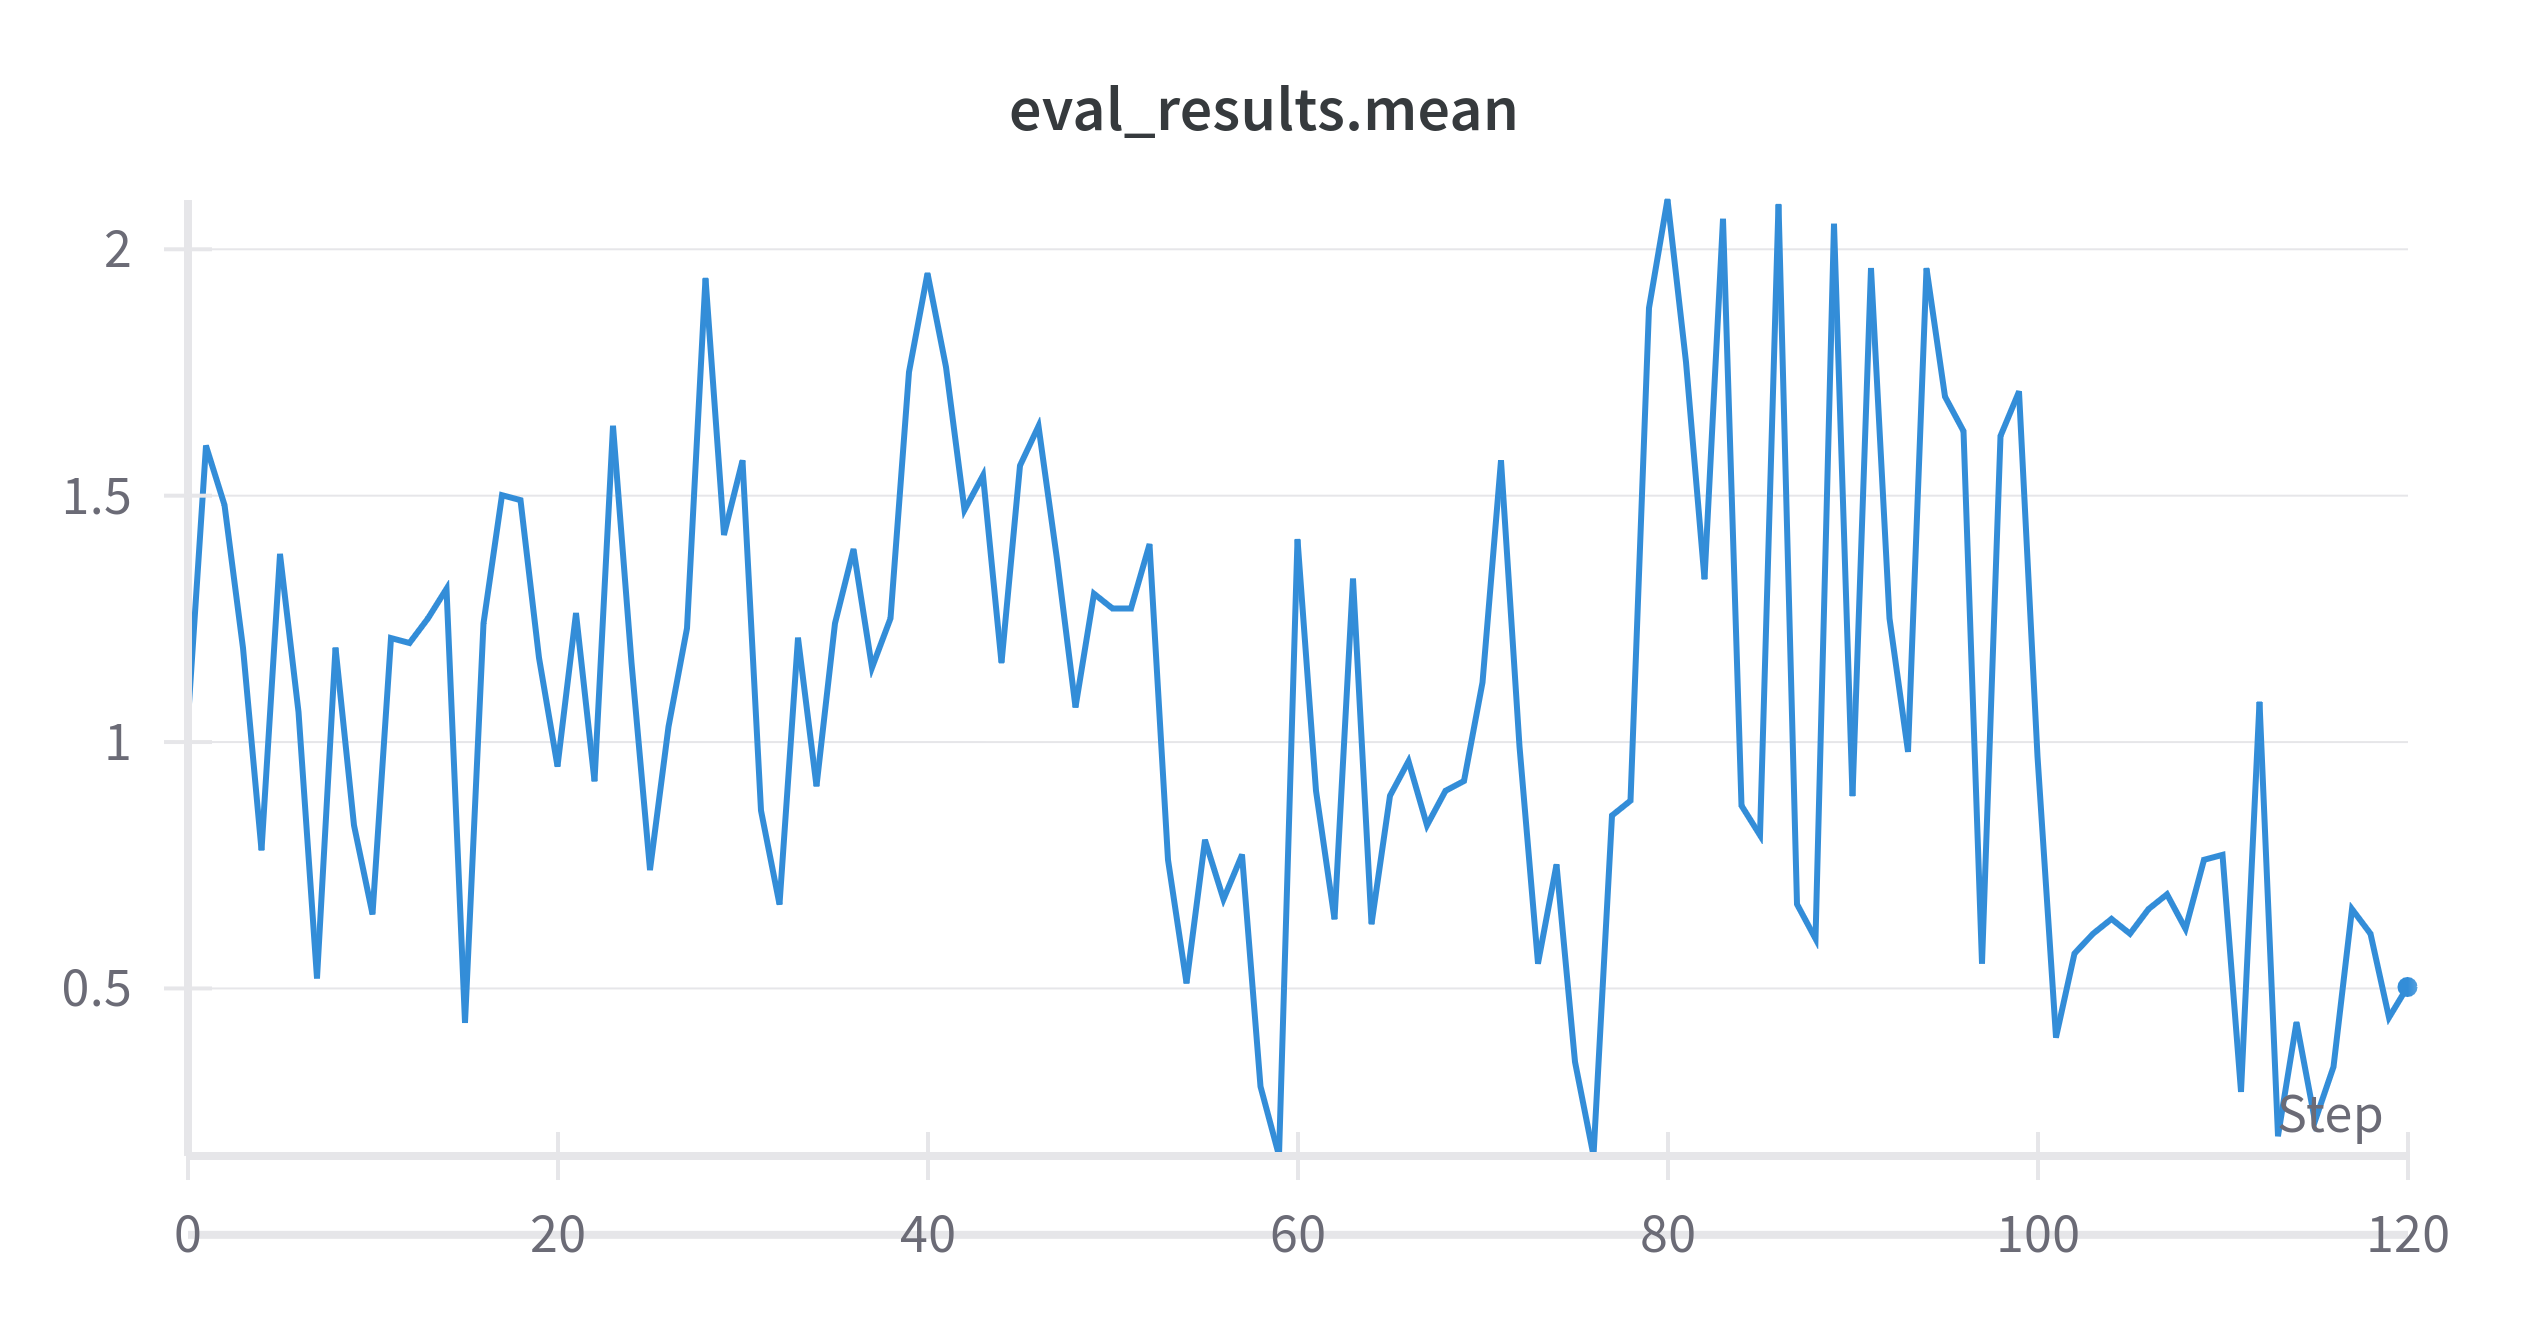
\includegraphics[width=\linewidth]{results/IQL.png}
  \caption{
    Training curve for Simple DQN Agent
  }
  \Description{Training curve for Simple DQN Agent}
  \label{fig:dqn}
\end{figure*}

\begin{figure*}[h]
  \centering
  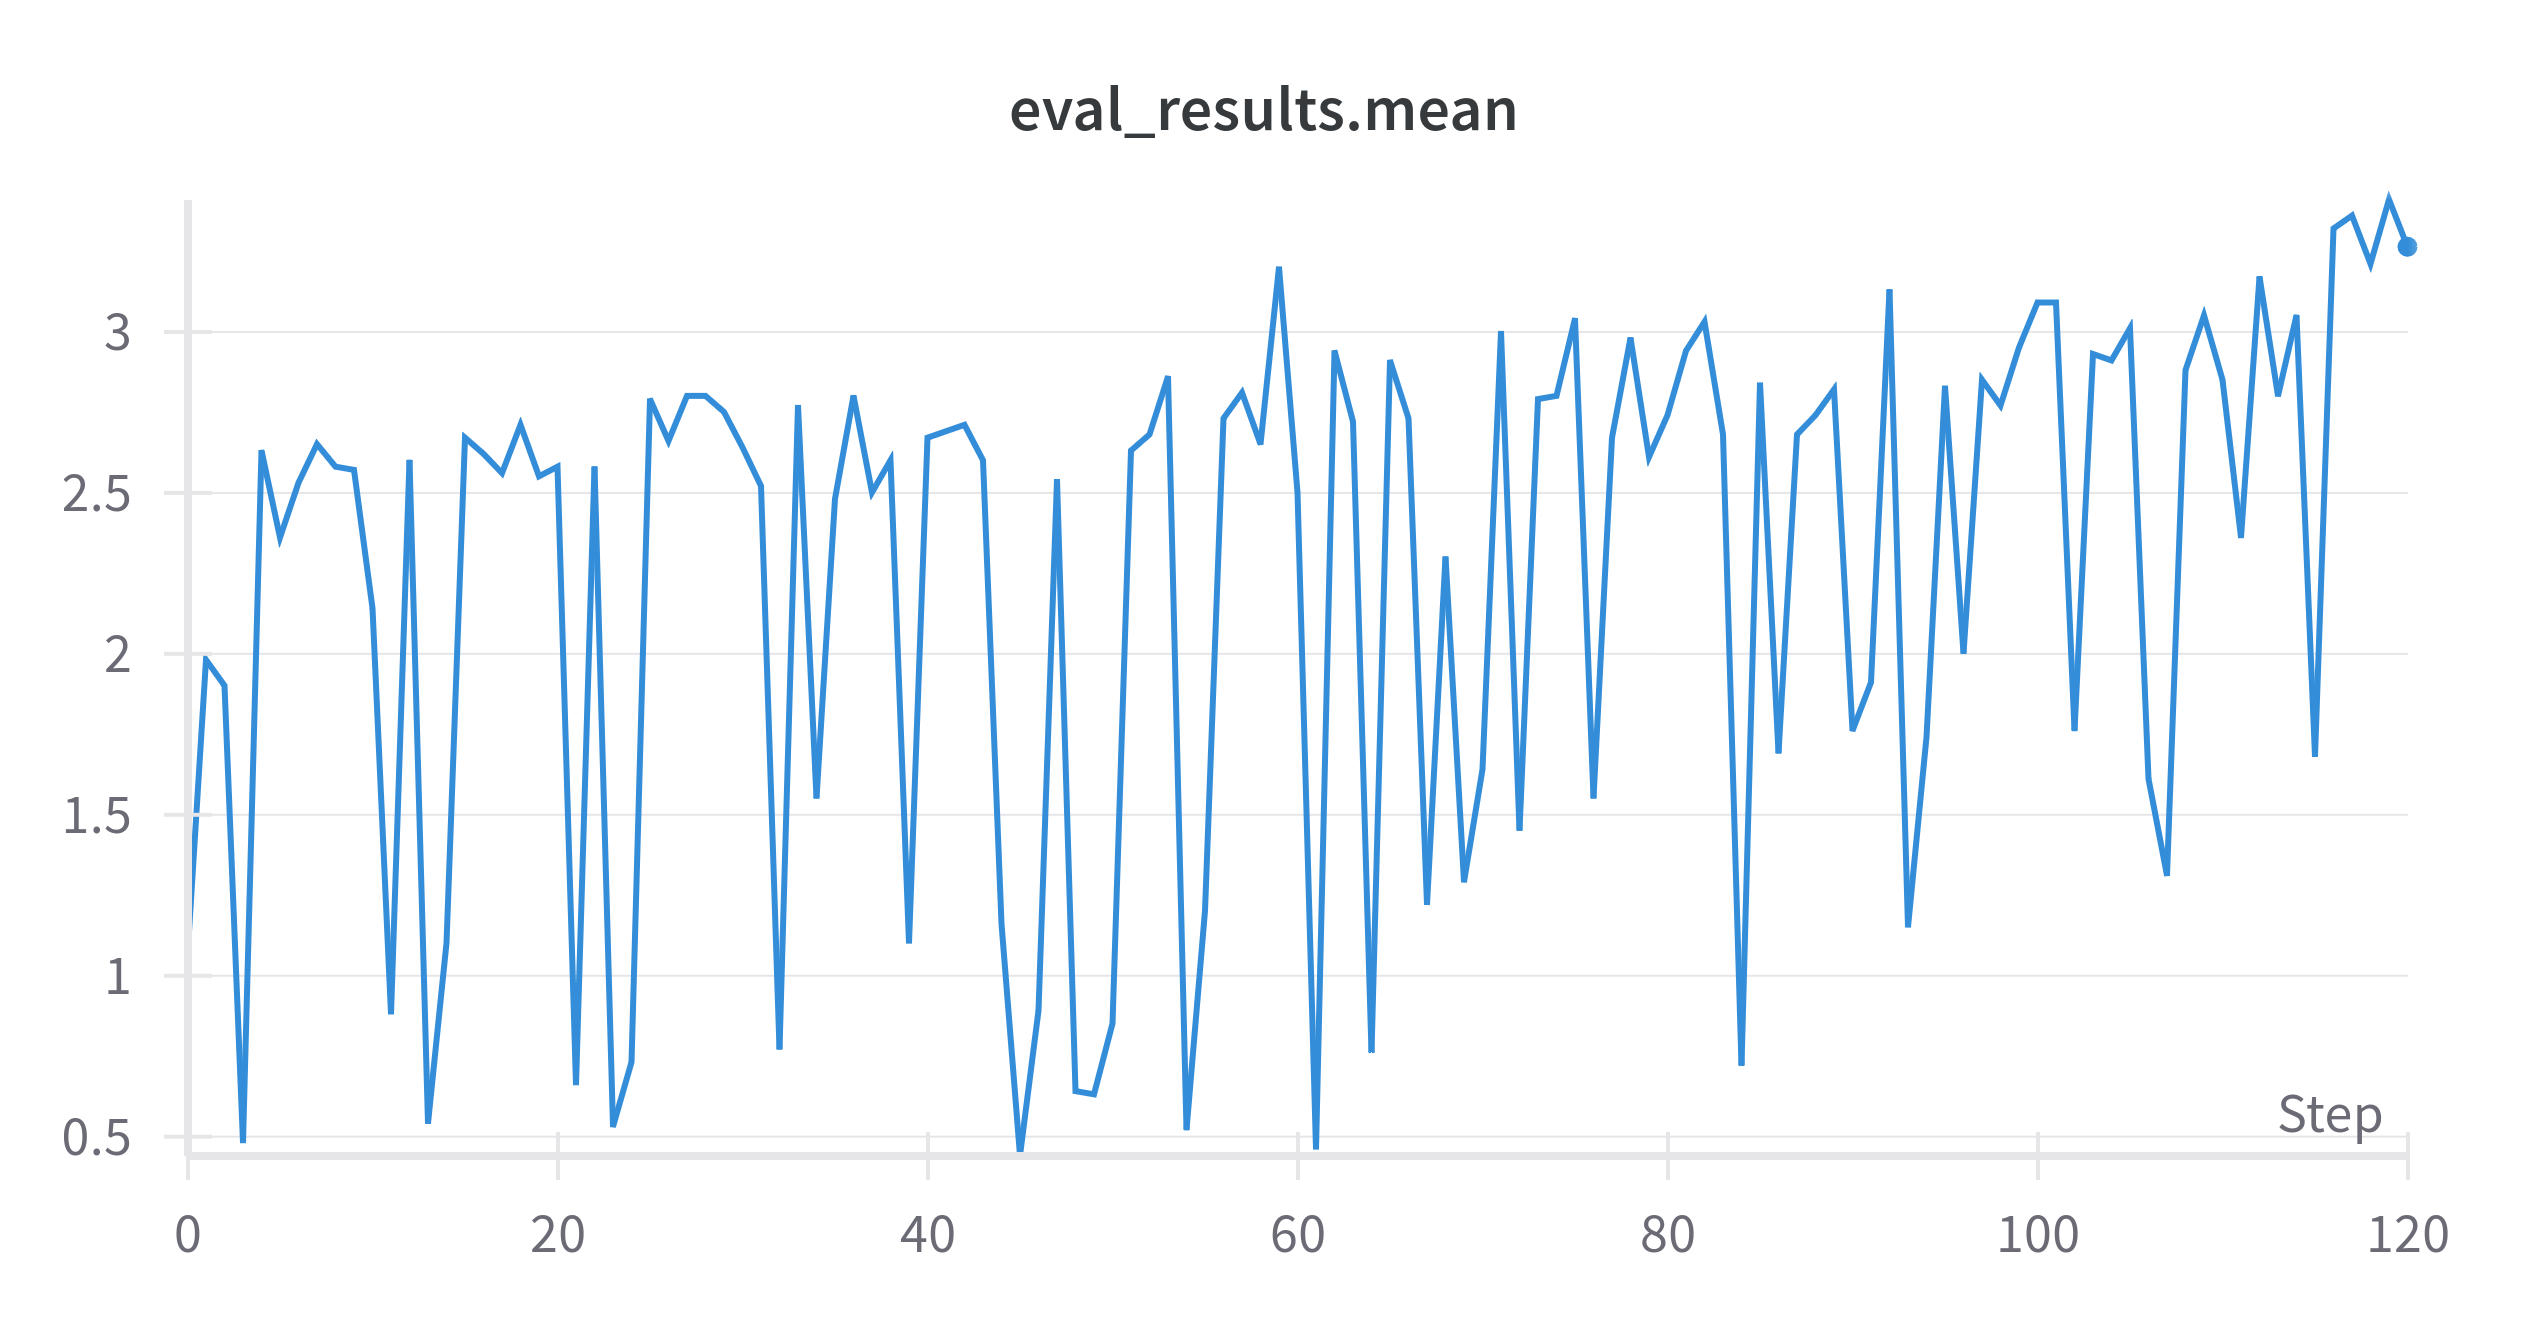
\includegraphics[width=\linewidth]{results/RAINBOW-mean.png}
  \caption{
    Training curve for Rainbow Agent
  }
  \Description{Training curve for Rainbow Agent}
  \label{fig:rainbow}
\end{figure*}

% \begin{figure*}[h]
%   \centering
%   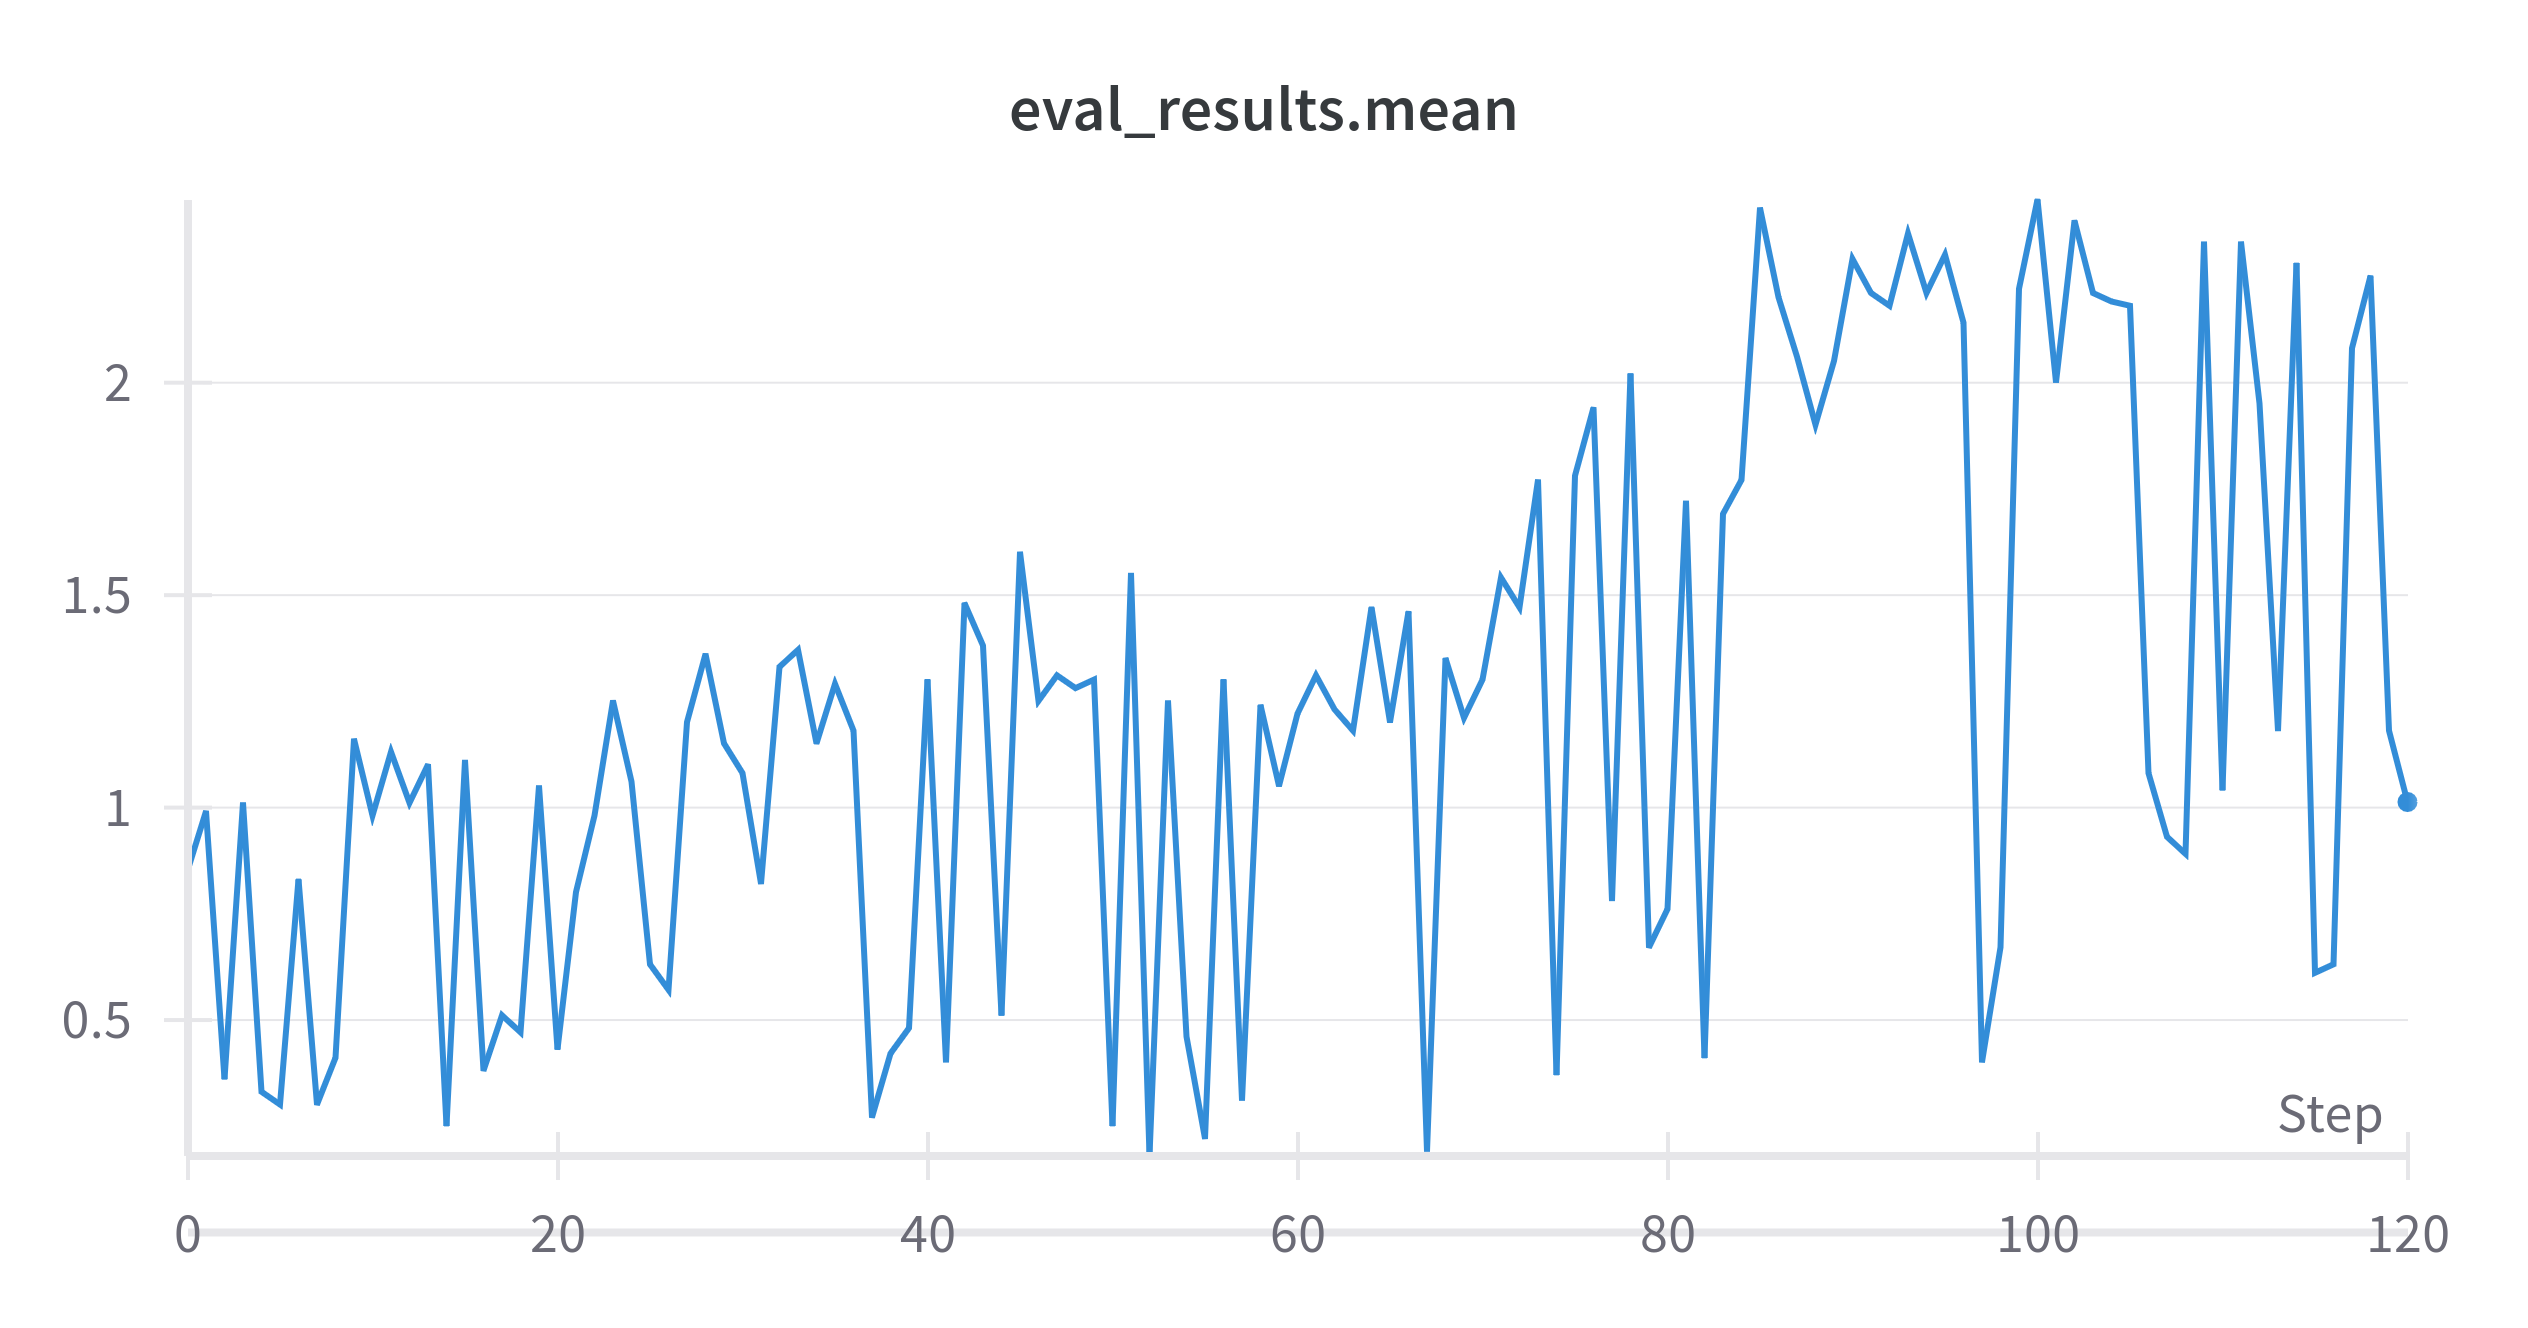
\includegraphics[width=\linewidth]{results/RAINBOW-3-mean.png}
%   \caption{
%     Training curve for Rainbow-3 Agent
%   }
%   \Description{Training curve for Rainbow-3 Agent}
% \end{figure*}

% \begin{figure*}[h]
%   \centering
%   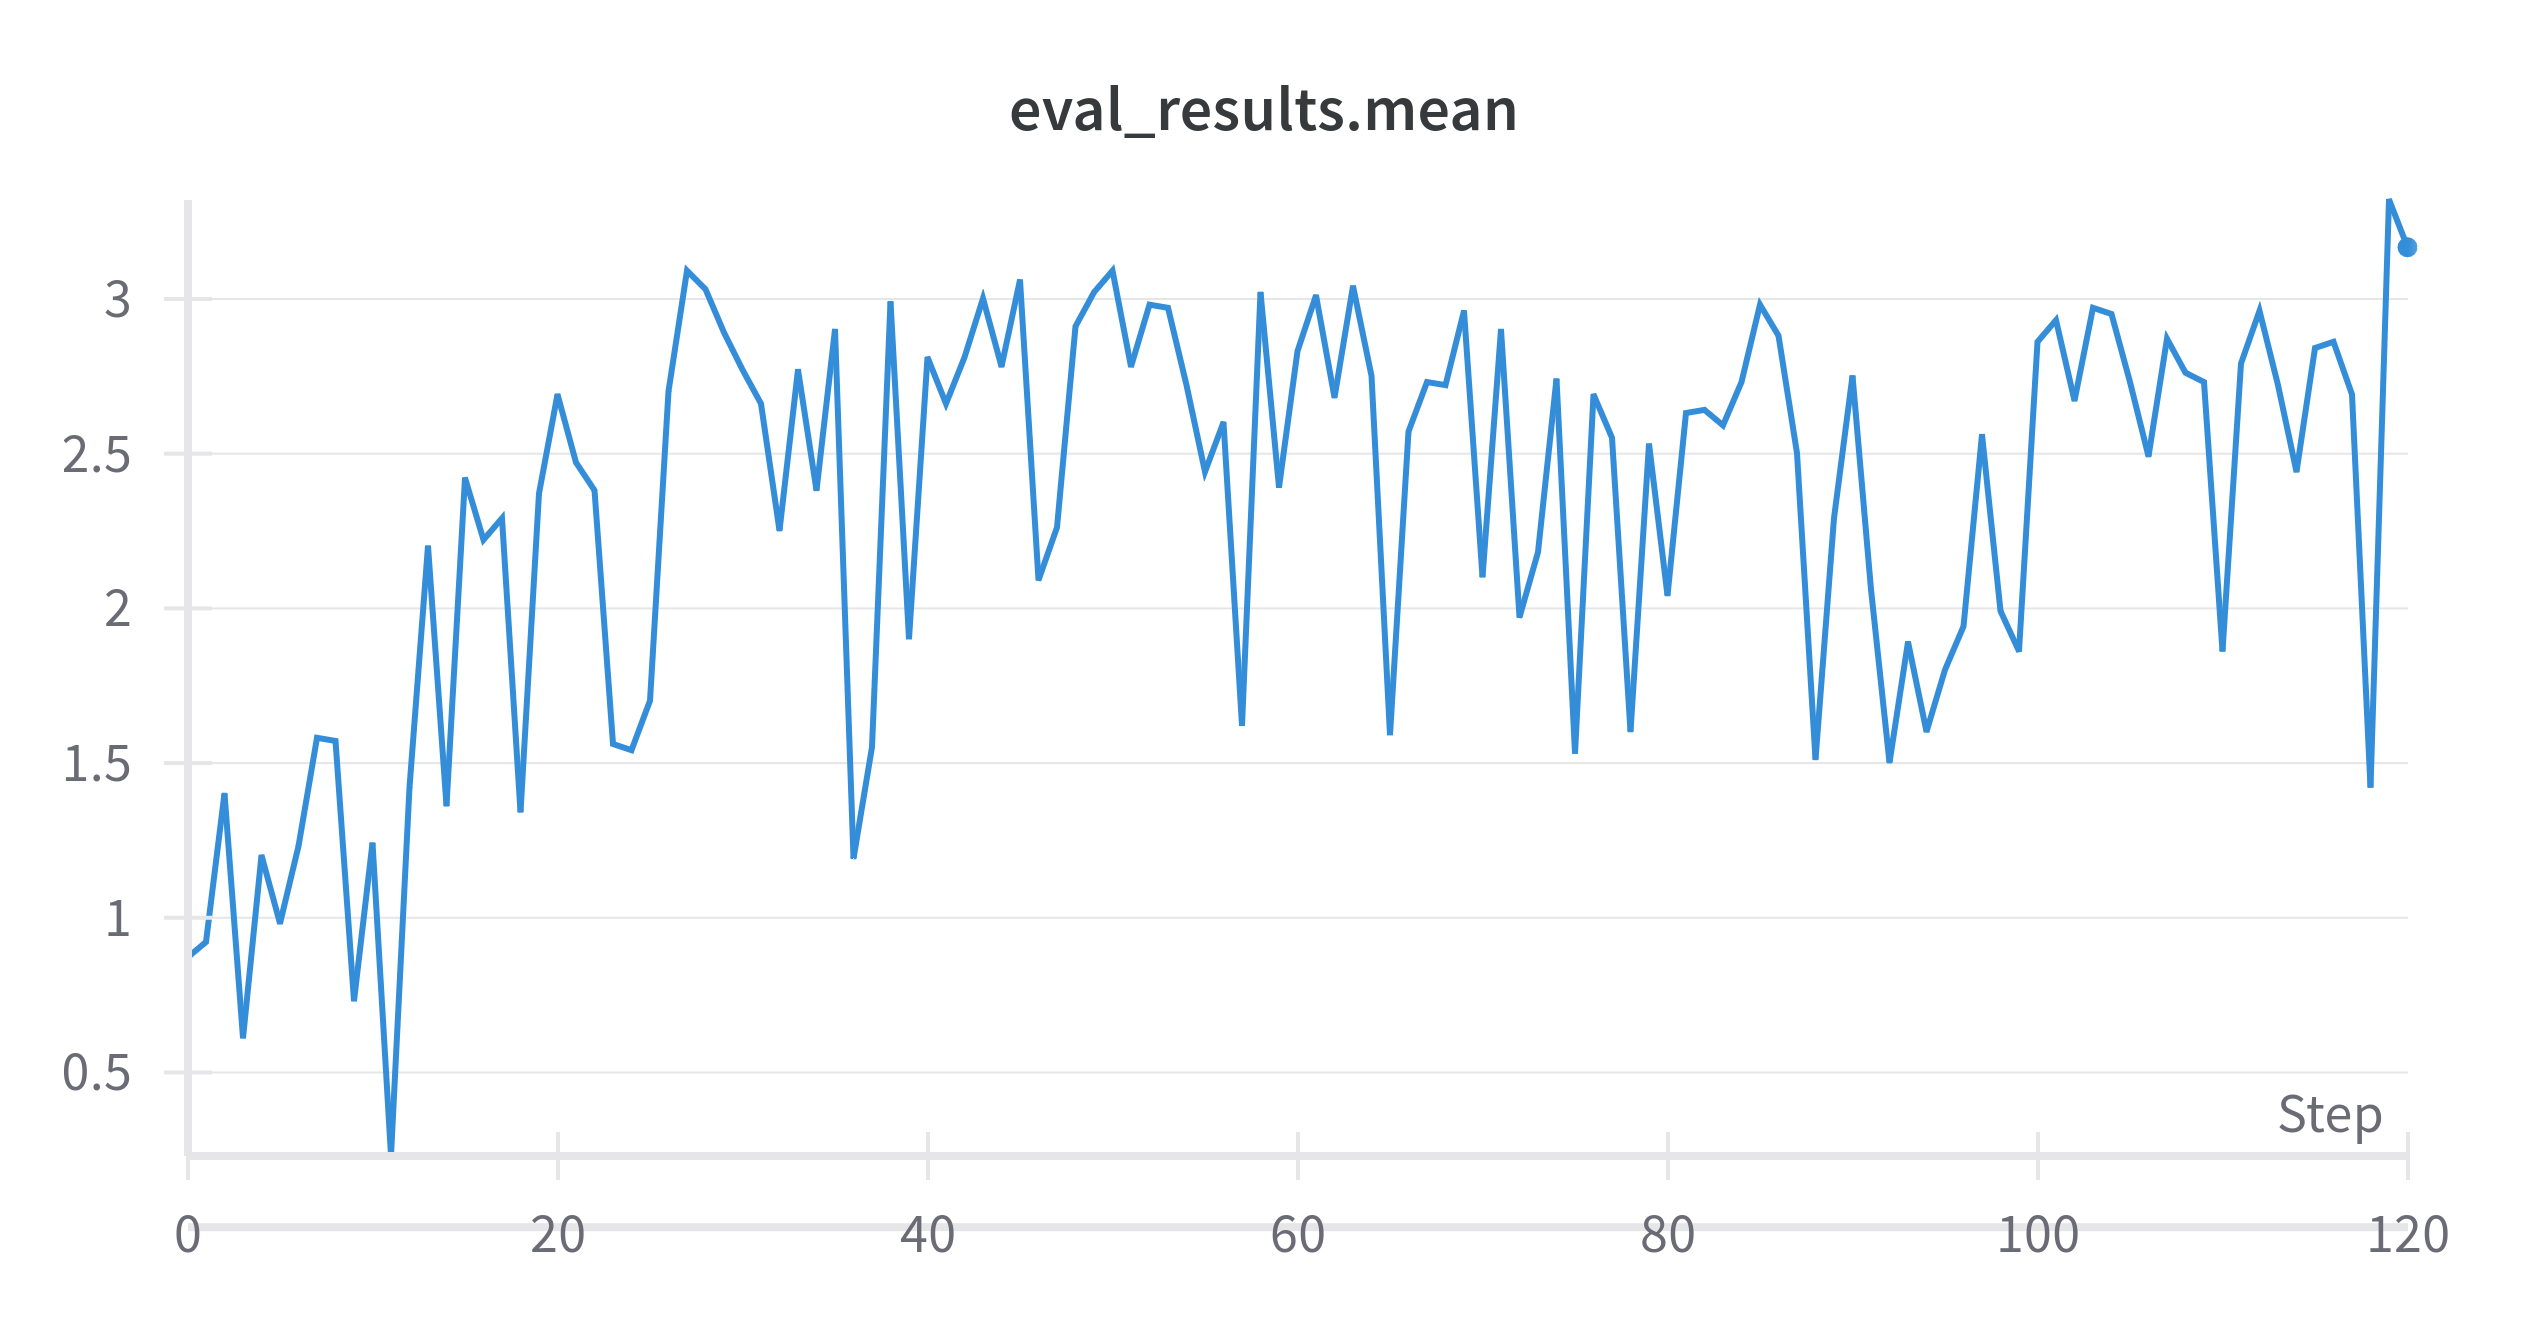
\includegraphics[width=\linewidth]{results/RAINBOW-5-mean.png}
%   \caption{
%     Training curve for Rainbow-5 Agent
%   }
%   \Description{Training curve for Rainbow-5 Agent}
% \end{figure*}


% \begin{figure*}[h]
%   \centering
%   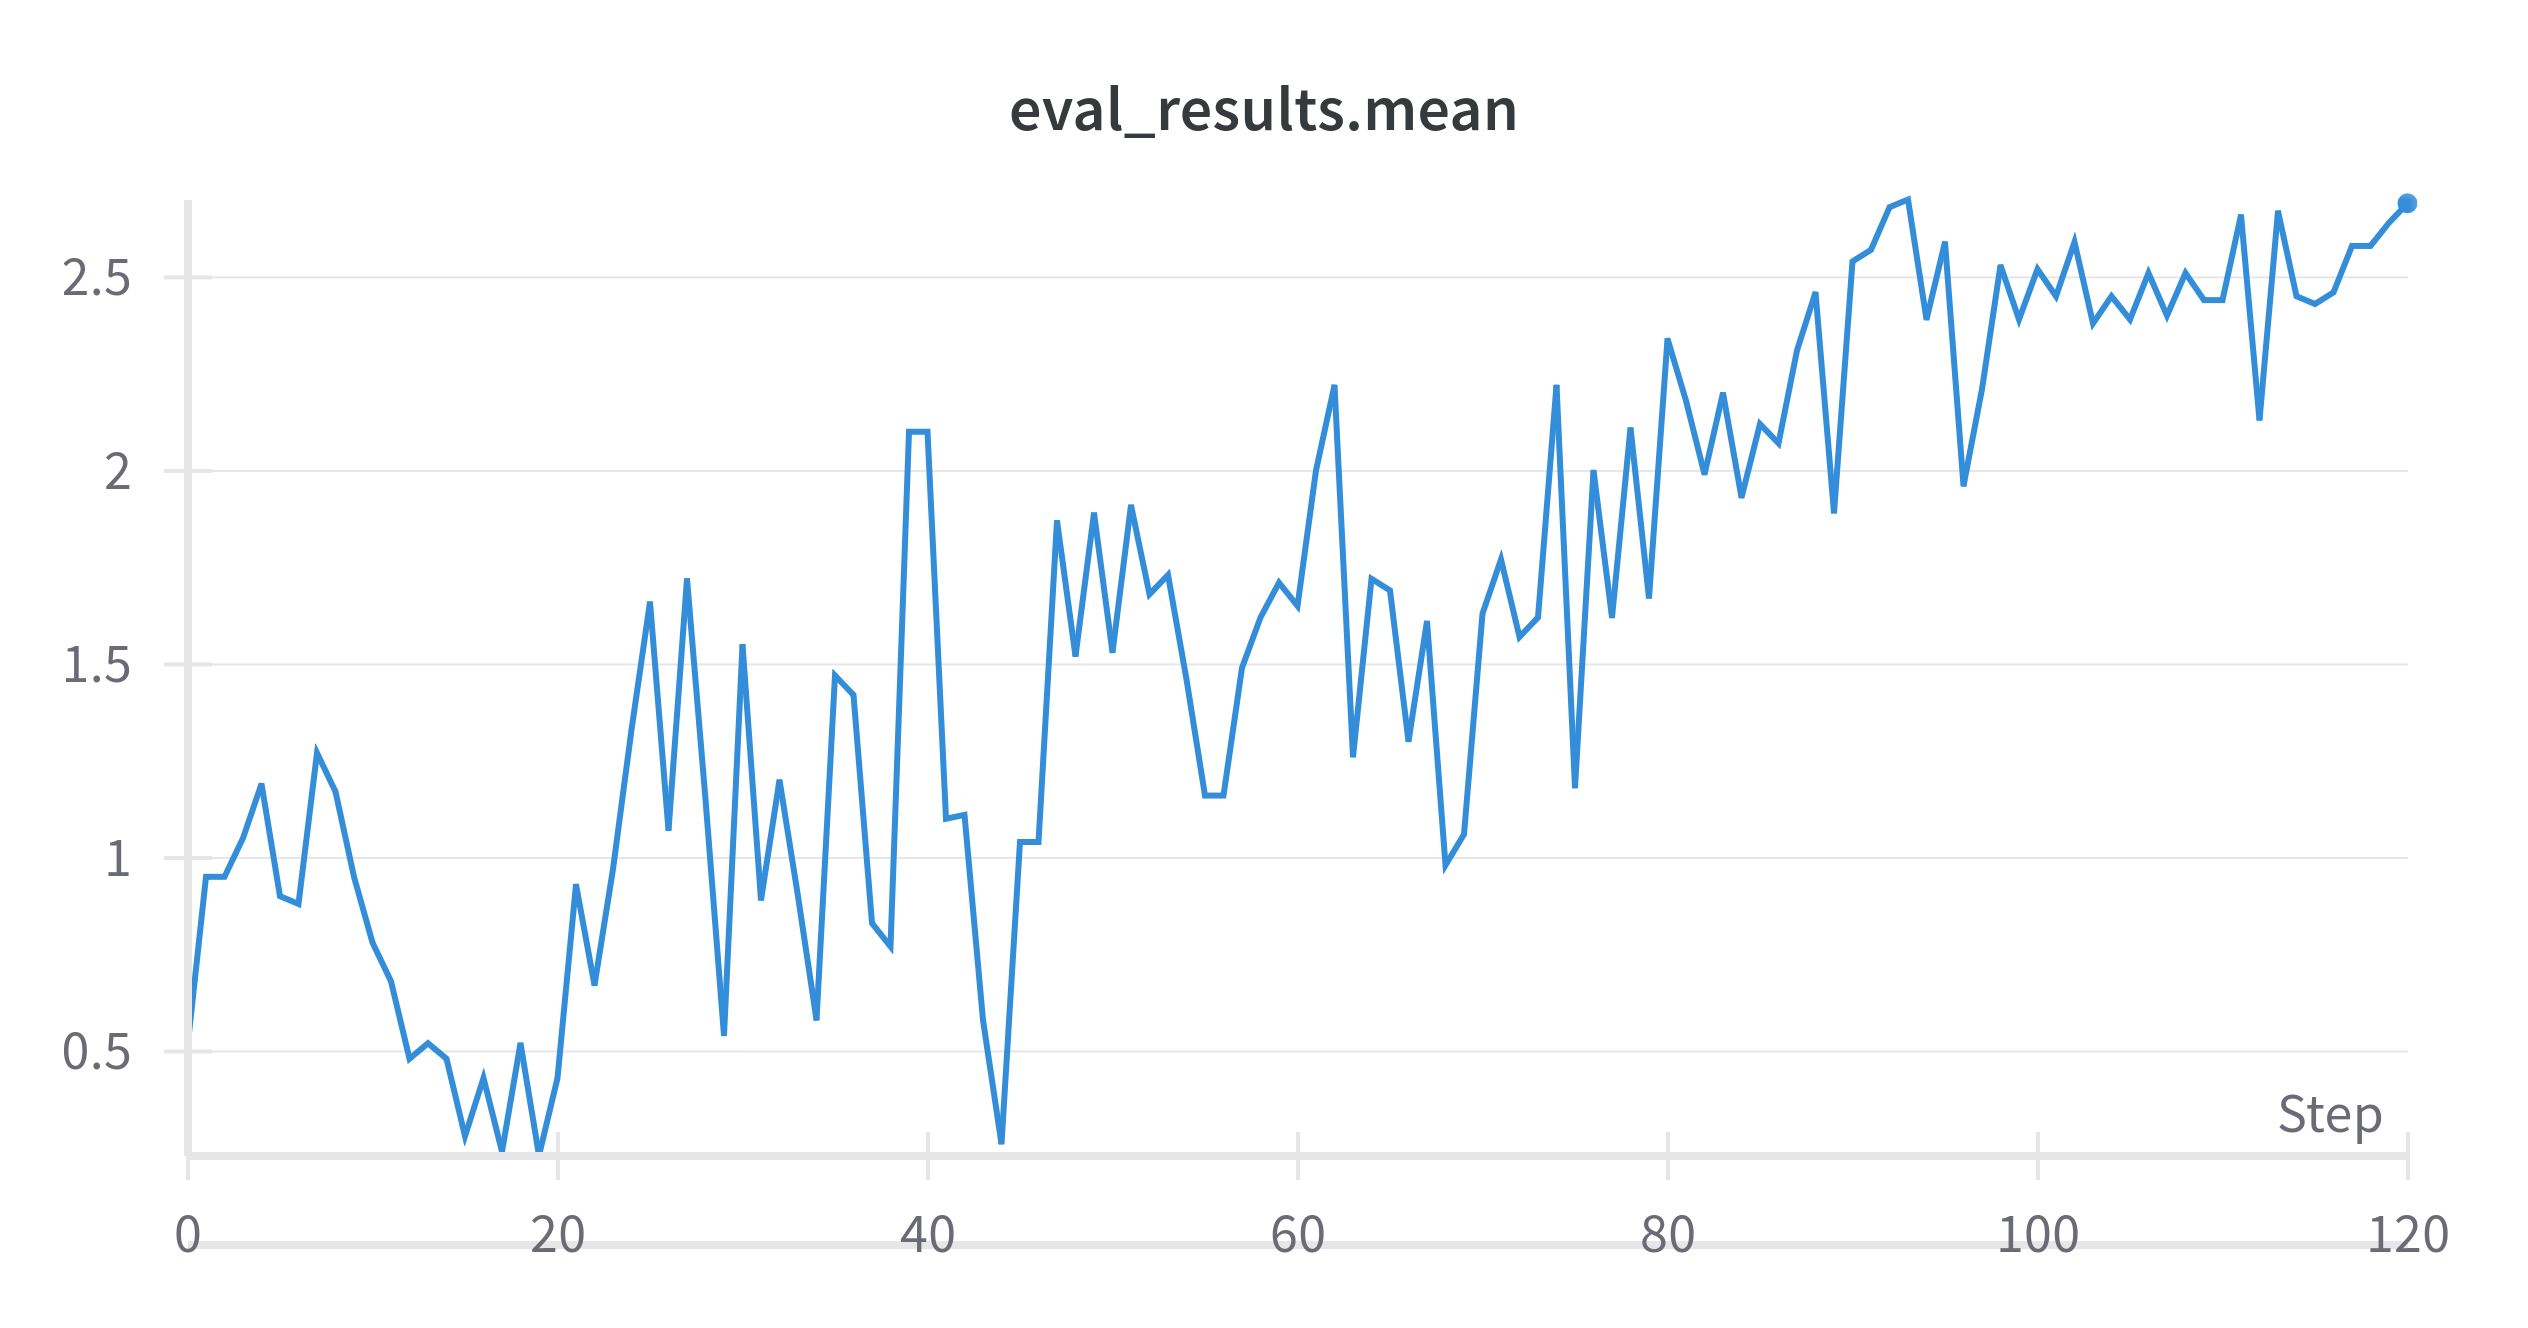
\includegraphics[width=\linewidth]{results/SAD-mean.png}
%   \caption{
%     Training curve for SAD Agent
%   }
%   \Description{Training curve for SAD Agent}
% \end{figure*}

\begin{figure*}[h]
  \centering
  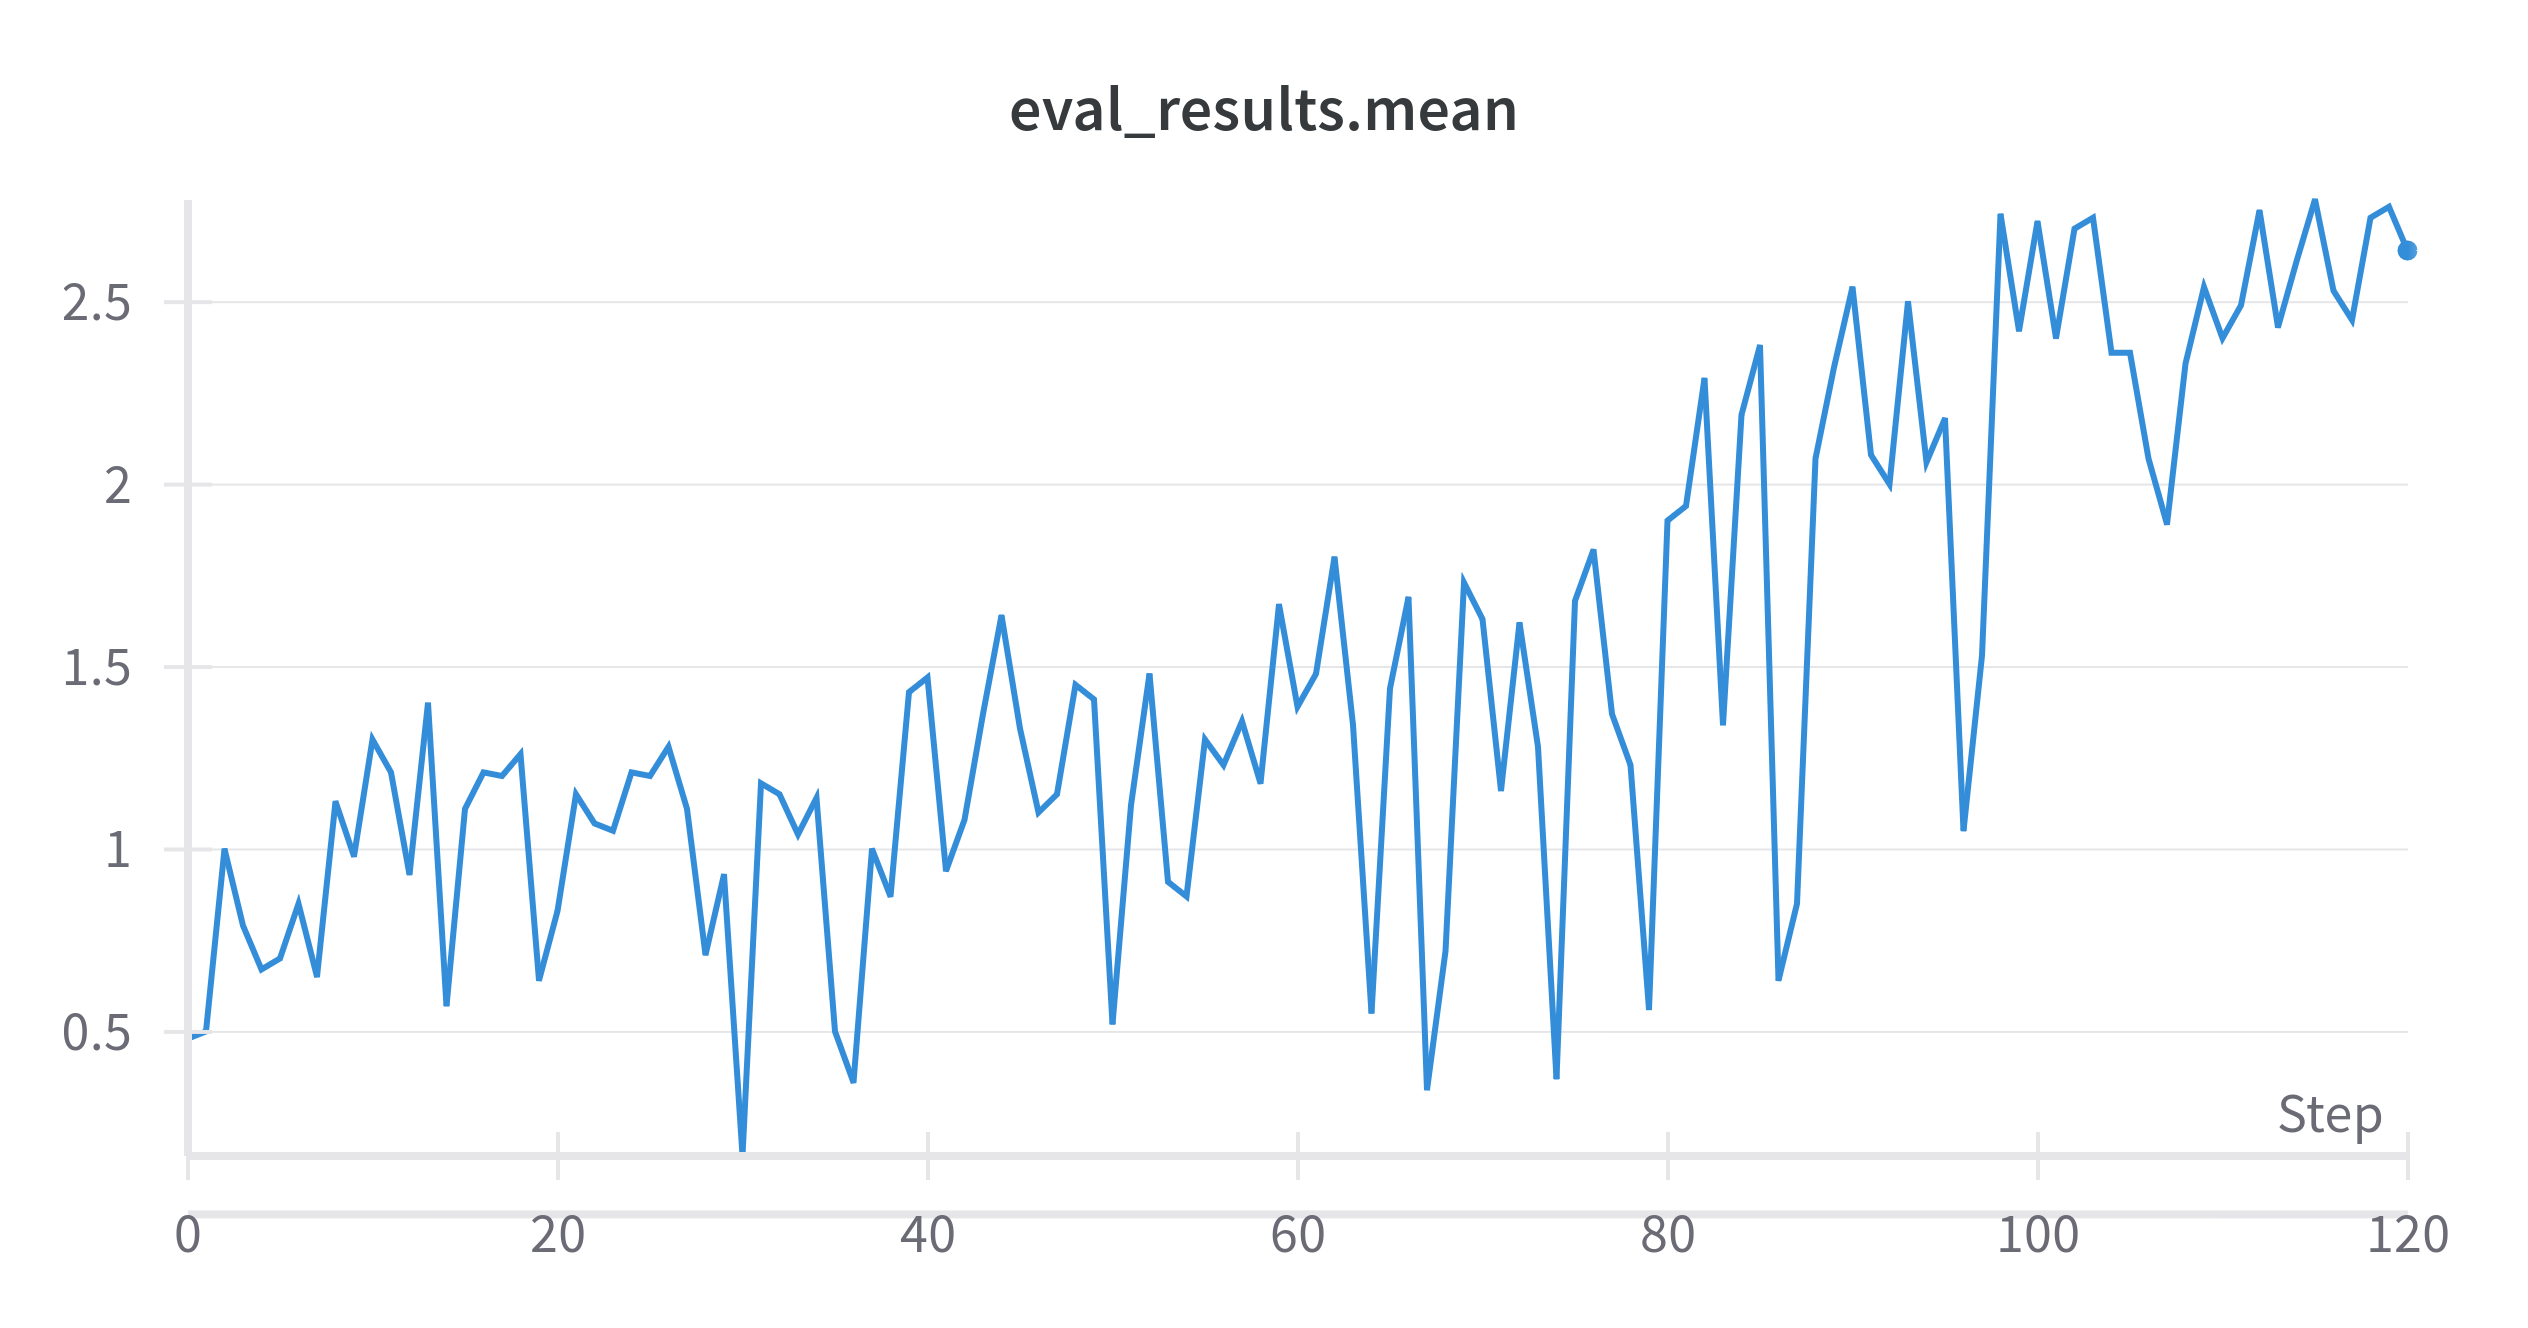
\includegraphics[width=\linewidth]{results/SAD-3-mean.png}
  \caption{
    Training curve for SAD-3 Agent
  }
  \Description{Training curve for SAD-3 Agent}
  \label{fig:sad3}
\end{figure*}
\begin{table*}
    \caption{Performance of learning agents in Cross-Play}
    \label{tab:xp_performance}
    \begin{tabular}{|c|c|c|c|c|c|c|c|c|}
      \toprule
        \textbf{Agent 1$\backslash$2}   &
        \textbf{Simple DQN}  &
        \textbf{Rainbow}     &
        \textbf{Rainbow-3}   &
        \textbf{Rainbow-5}   &
        \textbf{Distributed} &
        \textbf{SAD}         &
        \textbf{SAD-3}       &
        \textbf{Avg XP} \\
      \midrule
      \textbf{Simple DQN} &
        - &
        1.2(0.91) &
        0.78(0.92) &
        1.16(0.8) &
        0.53(0.8) &
        N/A &
        N/A &
        0.92(0.86) \\
      
        \textbf{Rainbow} &
        1.1(0.98) &
        - &
        1.49(1.6) &
        2.5(1.4) &
        1.36(1.36) &
        N/A &
        N/A &
        1.61(1.33) \\

        \textbf{Rainbow-3} &
        0.91(0.95) &
        1.56(1.59) &
        - &
        1.87(1.4) &
        1.07(1.3) &
        N/A &
        N/A &
        1.35(1.31) \\

        \textbf{Rainbow-5} &
        0.96(0.99) &
        2.39(1.43) &
        1.6(1.37) &
        - &
        1.18(1) &
        N/A &
        N/A &
        1.53(1.2) \\

        \textbf{Distributed} &
        1.25(1.02) &
        1.61(1.40) &
        1.26(1.31) &
        1.28(1.01) &
        - &
        N/A &
        N/A &
        1.35(1.19) \\

        \textbf{SAD} &
        N/A                  &
                N/A                  &
                N/A                  &
                N/A                  &
                N/A                  &
                -                    &
                2.4(1)               &
                2.4(1)
                \\ 



        \textbf{SAD-3}       &
        N/A                  &
        N/A                  &
        N/A                  &
        N/A                  &
        N/A                  &
        2.11(0.8)            &
        -                    &
        2.11(0.8)
        \\ 

        \textbf{Avg XP}      &
        1.01(0.99)           &
        1.69(1.33)           &
        1.28(1.3)            &
        1.7(1.15)            &
        1.04(1.12)           &
        2.11(0.8)            &
        2.4(1)               &
        \\ 
    \bottomrule
  \end{tabular}
  \end{table*}

\subsection*{Self-Play Performance}


Table~\ref{tab:sp_performance} shows the performance of the learning agents in the two-player self-play version of Hanabi. The agents are evaluated based on their ability to achieve a high score in the game. The final score is an average of the score achieved over 1000 episodes. The standard deviation of the final score is also included to show the stability of the learning process. See Appendix ~\ref{app:full_results} for the full results.

It is important to note that the rule-based approaches generally outperform the learning agents when considering sample-limited training, with only large-scale RL frameworks like R2D2+SAD \cite{huSimplifiedActionDecoder2021} and ACHA \cite{bardHanabiChallengeNew2020a} outperforming rule-based approaches.

We observe that none of the agents could achieve an average high score in the game. While not a focus of this study, we can attribute this to the sample's limited training setting and the higher complexity of the small version compared to the full game. 

The simple Dueling Double DQN fails to learn the game effectively and struggles to learn an optimal policy for the game. With a score of 0.502, we can conclude that the agent cannot play 1 card correctly on average. It is important to note that, at best, the agent can reach a score of 2.19 earlier in the training process, which shows some promise in the agent's ability to learn the game. However, the agent fails to maintain this performance and quickly regresses to a lower score. Without a clear trend in performance, we can conclude that the agent cannot effectively learn a policy for the game. This can be observed in Figure ~\ref{fig:dqn}.

The Rainbow DQN shows an impressive improvement in performance over the simple DQN agent, and we can identify a general improvement over time in its performance. However, we observe a cycle of regression and correction in the training, which we will discuss later.

When using a 1 step history, the Rainbow agent quickly learns a policy but then struggles to improve over time, likely due to the agent learning a suboptimal policy early in the game that it cannot recover from.

When using a 3 step history, we can identify an almost linear improvement in performance over time, with the agent quickly learning a policy and then steadily improving its performance. It performs slightly worse on average than the 1 step history but with a more stable learning curve. This is likely due to more samples being needed when looking at a longer history, which is a limitation of the sample-limited training setting. The final score of the agent is lower due to the aforementioned exploration regression cycle, but with more training, the agent would likely be able to achieve a higher score.

With a 5-step history, the results are similar to the 1-step history, with the agent quickly learning a policy but then struggling to improve over time. The agent receives a slightly lower score than the 1-step history, but due to the sample requirements of the longer history, the agent is likely to perform better with more training.

We compare these Rainbow results with a baseline Rainbow Agent with $\epsilon$-greedy exploration instead of Noisy Networks to evaluate the value of Noisy Network exploration. We find that the Noisy Network exploration is more sample efficient than $\epsilon$-greedy exploration, and the Rainbow agent can quickly achieve a significantly higher score without too much impact on the standard deviation. This is likely due to the Noisy Network exploration being more effective at exploring the state space of the game, and the agent can learn a more effective policy more quickly. However, we observe a cycle of regression and correction, observed in Figure ~\ref{fig:rainbow}, in the noisy network exploration agent. This is likely due to the agent learning a suboptimal policy and correcting itself in a cycle. This is a limitation of the exploration function of the agent, and the agent would likely be able to achieve a higher score and more stable learning curve with more training.

The simplified action decoder shows more stable learning and slightly lower performance than the Rainbow DQN agent. However, it showcases a nearly linear improvement in performance over time with a stable and consistent learning curve. When looking at a 3-step history, observed in Figure ~\ref{fig:sad3}, this improvement is more pronounced. SAD, however, slightly decreases the performance of the agent when compared to the baseline Rainbow DQN agent. This is likely due to the additional information provided to the agent during training, which increases the complexity of the learning process.

The stable training curve and lower standard deviation in the final score outline the value of the SAD algorithm in learning the partnership dynamics of the game more effectively. The SAD algorithm can model the other policy effectively and learn more efficiently from it. This is important as in a game like Hanabi, the partnership dynamics are crucial to achieving a high score.

In the literature, the SAD algorithm has been shown to outperform the Rainbow DQN algorithm in the two-player self-play version of Hanabi \cite{huSimplifiedActionDecoder2021}. However, in this study, the Rainbow DQN algorithm can outperform the SAD algorithm. In the literature, the SAD algorithm is often trained in an unlimited sample setting, with a combination of distributed reinforcement learning and recurrent experience replay. This is likely the reason for the discrepancy in performance between the two algorithms. The SAD algorithm is likely to perform better with more training but, in a sample-limited setting, is less effective than the Rainbow DQN algorithm.

\subsection*{AD-Hoc Teamplay Performance}

Table ~\ref{tab:xp_performance} shows the performance of learning agents in the AD-Hoc Teamplay setting.

By observing the decrease in the average score (Avg XP) and increase in the standard deviation of the final score, we find that all the agents struggle to cooperate effectively in cross-play (XP) settings, except for the simple DQN, which seems to improve, which can be attributed to the skill of its partners. The general decrease in the score and increase in the standard deviation is likely due to the agents learning arbitrary conventions that are specific to their partners during training, or "idiosyncratic conventions" as described by \textcite{lucasAnyPlayIntrinsicAugmentation2022}. This is a significant limitation of the current state-of-the-art in Hanabi, and it raises the importance of finding sample-efficient algorithms for Hanabi that can generalize to new partners.

